\documentclass{article}
\begin{document}
\subsection{Running example on MCU side}
Here are the step-by-step instructions to run examples on MCU side:
\begin{itemize}
	\item Selected Platform: Windows
	\item Board: APP3.1
	\item Sensor shuttle: BMI270
	\item Example: \path{\examples\bmi270\bmi270_examples\accel_gyro}
\end{itemize}
\begin{enumerate}
	\item Connect the Application Board board via USB, with the sensor shuttle board mounted.
	\item Open the command prompt or the terminal.
	\item Use the command \texttt{cd} to go to the directory where the example that is to be built is located.
	\begin{figure}[H]
		\begin{center}
			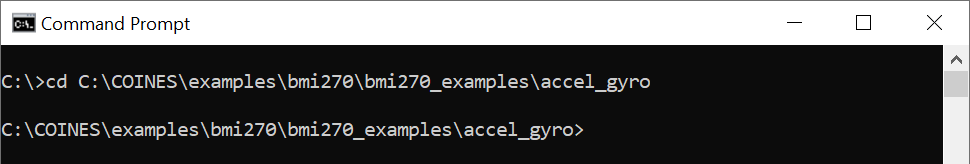
\includegraphics[width=0.9\textwidth]{coinesAPI_images/Mcu_example_cd.png}
		\end{center}
	\end{figure}
	\item Execute command "mingw32-make TARGET=MCU\_APP31 download"
	\begin{figure}[H]
		\begin{center}
			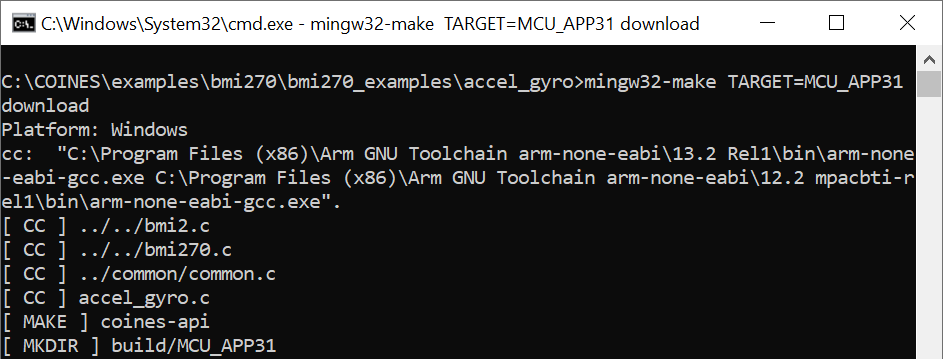
\includegraphics[width=0.9\textwidth]{coinesAPI_images/Mcu_example_compile.png}
		\end{center}
	\end{figure}
	\begin{figure}[H]
		\begin{center}
			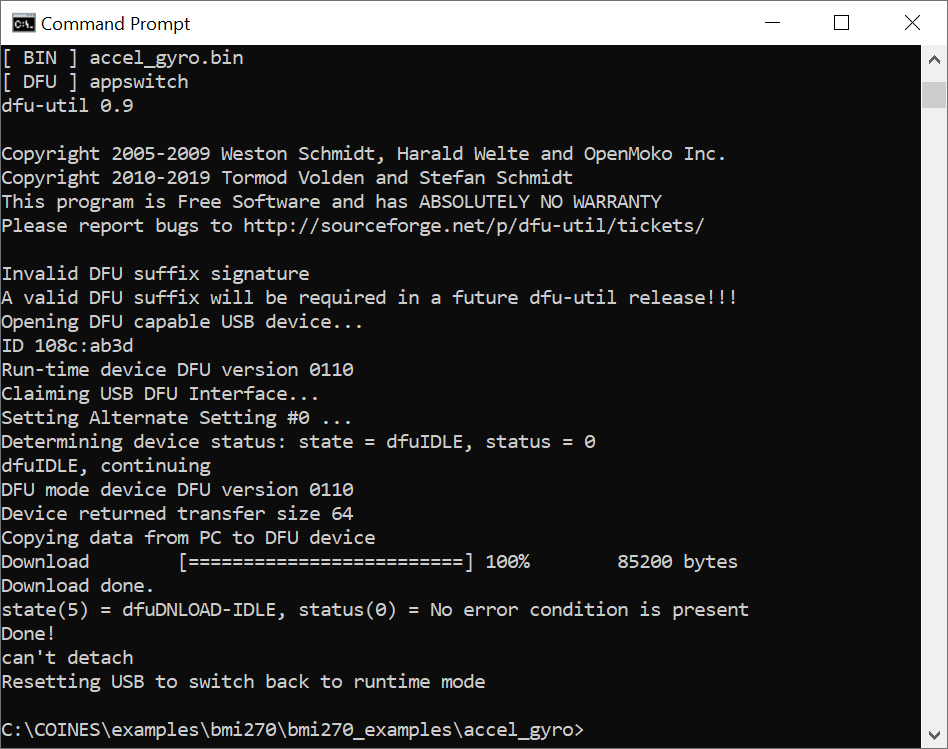
\includegraphics[width=0.9\textwidth]{coinesAPI_images/Mcu_example_download.png}
		\end{center}
	\end{figure}
	\item View the output in a serial terminal application like HTerm
	\begin{figure}[H]
		\begin{center}
			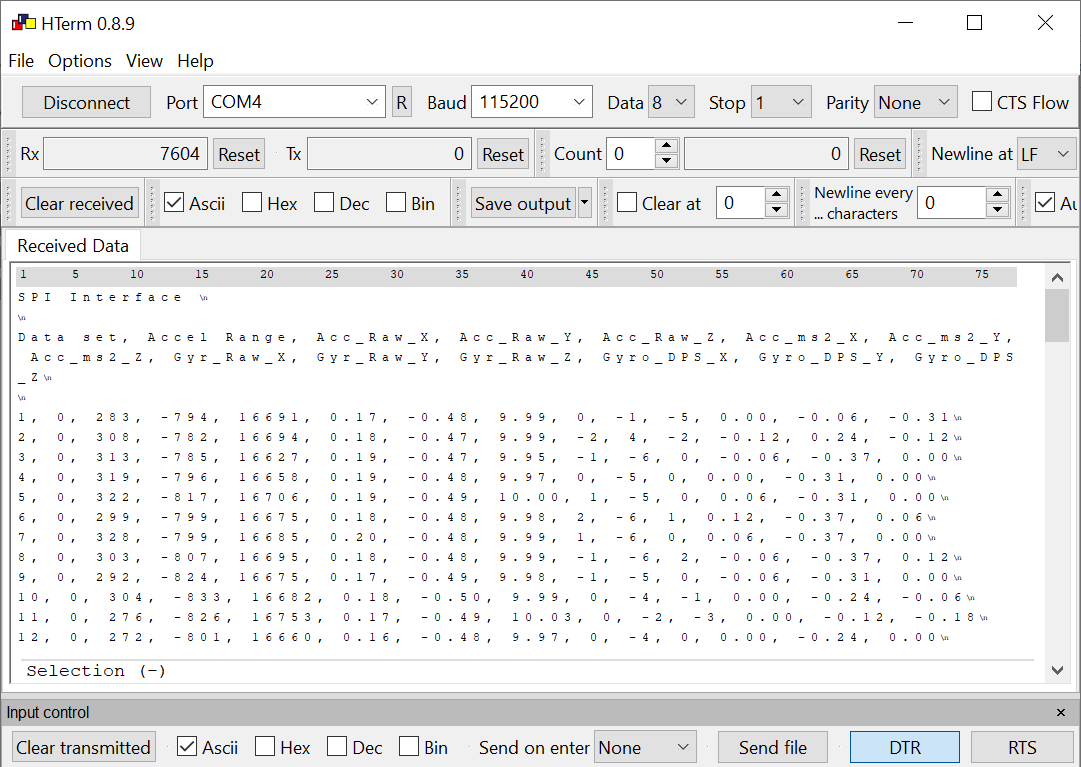
\includegraphics[width=0.9\textwidth]{coinesAPI_images/Mcu_example_output.png}
		\end{center}
	\end{figure}
	\begin{figure}[H]
		\begin{center}
			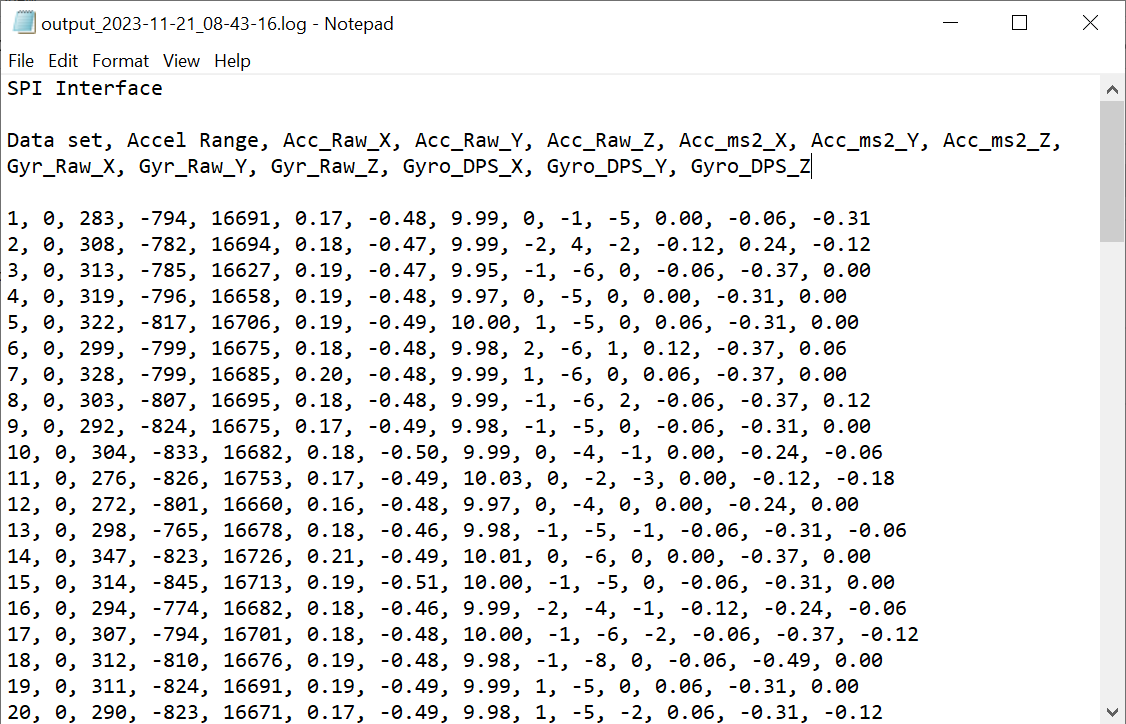
\includegraphics[width=0.9\textwidth]{coinesAPI_images/Mcu_example_log.png}
		\end{center}
	\end{figure}
\end{enumerate}

\end{document}